\documentclass[svgnames,envcountsame,envcountsect,envcountreset]{llncs}
\usepackage{preamble} 
\let\extendedversion\relax % uncomment for extended version - AC
\input{macros}
\pagestyle{plain}
% 
\begin{document} 
% 

bkla bla bla 


\usetikzlibrary{calc}

% % #1 = marked corner node
% % #2 = opposite node in the square
% % #3 = position along diagonal (0..1)
% % #4 = arm length (dimension, e.g. 3mm, 4pt, 0.2cm)
% \newcommand{\pushoutmark}[4]{%
%   \draw
%     let
%       \p1 = (#1),
%       \p2 = (#2),
%       \p3 = ($(#1)!#3!(#2)$),
%       \n1 = {ifthenelse(\x2>\x1, -1, 1)}, % x sign toward opposite
%       \n2 = {ifthenelse(\y2>\y1, -1, 1)}  % y sign toward opposite
%     in
%       (\p3) -- ++({\n1*(#4)},0) -- (\p3) -- ++(0,{\n2*(#4)});
% }

\begin{tikzpicture}[>=Stealth]
  \node (A) at (0,1) {$A$};
  \node (B) at (2,1) {$B$};
  \node (C) at (0,0) {$C$};
  \node (D) at (2,0) {$D$};

  \draw[->] (A)--(B);
  \draw[->] (A)--(C);
  \draw[->] (B)--(D);
  \draw[->] (C)--(D);

  \pushoutmark{D}{A}{0.25}{2mm}
\end{tikzpicture}


\begin{equation}\label{eq:pushout} % pushout
    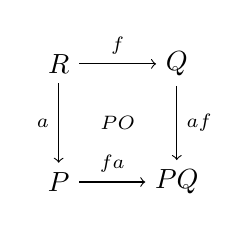
\begin{tikzpicture}[auto,node distance = 1.5cm]
      \node (R) {$R$};
      \node (Q) [right of=R] {$Q$};
      \node (P) [below of=R] {$P$};
    \node (PO) [below of=Q] {$P\tdarr Q$};

    \path
      (R) edge [->] node[auto] {$\scriptstyle{f}$}  (Q)
      edge [->] node[auto,swap] {$\scriptstyle{a}$}  (P)
    (Q) edge [->] node[auto] {$\scriptstyle{a\tdarr f}$}  (PO)
    (P) edge [->] node[auto] {$\scriptstyle{f\tdarr a}$}  (PO); 
\draw (.75,-.75) node {$\scriptstyle{PO}$};
\pushoutmark{PO}{R}{0.25}{2mm}
    \end{tikzpicture}
  \end{equation} 

%   \begin{equation}\label{eq:pushout}
%     \begin{tikzpicture}[auto,node distance = 1.5cm]
%       \node (R) {$R$};
%       \node (Q) [right of=R] {$Q$}
%       edge [<-] node[auto,swap] {$\scriptstyle{f}$}  (R);
%       \node (P) [below of=R] {$P$}
%       edge [<-] node[auto] {$\scriptstyle{a}$}  (R);
%       \node (PO) [below of=Q] {$P\tdarr Q$}
% edge [<-] node[auto,swap] {$\scriptstyle{a\tdarr f}$}  (Q)
% edge [<-] node[auto,swap] {$\scriptstyle{f\tdarr a}$}  (P); 
% \draw (.75,-.75) node {$\scriptstyle{PO}$};
%     \end{tikzpicture}
%   \end{equation} 

\begin{equation} % true
  \begin{tikzpicture}[node distance = 1.5cm]
      \node (R) {$\disc{\varnothing}$};
      \node (G) [right of=R] {$G$};
      \node (P) [below of=R] {$\disc{\varnothing}$};
      \tri{R}{1.8}{1}{2}{}
      \node (lab) [above of=R-left, xshift=-3mm, yshift=-5mm] {$\scriptstyle{\abc{\True}}$};

      \path
        (R) edge [->] node[auto] {$\scriptstyle{g}$}  (G)
         edge [->] node[auto,swap] {$\scriptstyle{id}$}  (P)
        (P) edge [->] node[auto,swap] {$\scriptstyle{g}$}  (G);
    \end{tikzpicture}
 \end{equation} 

 \begin{equation} % true completo
  \begin{tikzpicture}[node distance = 1.5cm]
      \node (R) {$\disc{\varnothing}$};
      \node (G) [right of=R] {$G$};
      \node (P) [below of=R] {$\disc{\varnothing}$};
      \tri{R}{2.1}{1}{2}{}
      \node (lab) [above of=R-left, xshift=-3mm, yshift=-5mm] {$\scriptstyle{\abc{\True}}$};
      

      \path
        (R) edge [->] node[auto] {$\scriptstyle{g}$}  (G)
         edge [->] node[xshift=-2mm] {$\scriptstyle{id}$}  (P)
        (P) edge [->] node[auto,swap] {$\scriptstyle{g}$}  (G);
        \tri{P}{0.5}{0.3}{0.6}{}
    \end{tikzpicture}
 \end{equation} 


% \begin{equation} % true
%   \begin{tikzpicture}[auto,node distance = 1.5cm]
%       \node (R) {$\disc{\varnothing}$};
%       \node (G) [right of=R] {$G$}
%       edge [<-] node[auto,swap] {$\scriptstyle{g}$}  (R);
%       \node (P) [below of=R] {$\disc{\varnothing}$}
%       edge [<-] node[auto] {$\scriptstyle{id_{\disc{\varnothing}}}$}  (R)
%       edge [->] node[auto,swap] {$\scriptstyle{g}$}  (G);
%     \end{tikzpicture}
%  \end{equation} 

 \begin{equation} % x = y 
  \begin{tikzpicture}[node distance = 1.5cm]
    \node (R) {$\disc{{{\{x,y\}}}}$};
    \node (G) [right of=R] {$G$};
    \node (P) [below of=R] {$\disc{{{\{z\}}}}$};
    \tri{R}{2.1}{1}{2}{}
\node (lab) [above of=R-left, xshift=-3mm, yshift=-5mm] {$\scriptstyle{\abc{x\Eq y}}$};
    \path
        (R) edge [->] node[auto] {$\scriptstyle{g}$}  (G)
         edge [->] node {${\begin{aligned}\scriptstyle{x\mapsto z}\\[-2ex]
         \scriptstyle{y\mapsto z}\end{aligned}}$}  (P)
      (P) edge [->] node[auto,swap] {$\scriptstyle{h}$}  (G);
      \tri{P}{0.5}{0.3}{0.6}{}
    \end{tikzpicture}
 \end{equation} 

%  \begin{equation} % x = y 
%   \begin{tikzpicture}[auto,node distance = 1.5cm]
%       \node (R) {$\disc{{{\{x,y\}}}}$};
%       \node (G) [right of=R] {$G$}
%       edge [<-] node[auto,swap] {$\scriptstyle{g}$}  (R);
%       \node (P) [below of=R] {$\disc{{{\{z\}}}}$}
%       edge [<-] node[auto] {${\begin{aligned}\scriptstyle{x\mapsto z}\\[-2ex]
%          \scriptstyle{y\mapsto z}\end{aligned}}$}  (R)
%       edge [->] node[auto,swap] {$\scriptstyle{h}$}  (G);
%     \end{tikzpicture}
%  \end{equation} 

 \begin{equation} % a(x,y)
  \begin{tikzpicture}[node distance = 1.5cm]
      \node (R) {$\disc{{{\{x,y\}}}}$};
      \node (G) [right of=R] {$G$};
      \node[graph] (P) [below of=R] {$\scriptstyle{\oneedge{x'}{a}{y'}}$};
      \tri{R}{2.1}{1.2}{2.4}{}
\node (lab) [above of=R-left, xshift=-3mm, yshift=-5mm] {$\scriptstyle{\abc{\la(x,y)}}$};

      \path
        (R) edge [->] node[auto] {$\scriptstyle{g}$}  (G)
        edge [->] node {${\begin{aligned}\scriptstyle{x\mapsto x'}\\[-2ex]
         \scriptstyle{y\mapsto y'}\end{aligned}}$}  (P)
        (P) edge [->] node[auto,swap] {$\scriptstyle{h}$}  (G); \tri{P}{0.5}{0.3}{0.6}{}
    \end{tikzpicture}
 \end{equation} 

%  \begin{equation} % a(x,y)
%   \begin{tikzpicture}[auto,node distance = 1.5cm]
%       \node (R) {$\disc{{{\{x,y\}}}}$};
%       \node (G) [right of=R] {$G$}
%       edge [<-] node[auto,swap] {$\scriptstyle{g}$}  (R);
%       \node[graph] (P) [below of=R] {$\scriptstyle{\oneedge{x'}{a}{y'}}$}
%       edge [<-] node[auto] {${\begin{aligned}\scriptstyle{x\mapsto x'}\\[-2ex]
%          \scriptstyle{y\mapsto y'}\end{aligned}}$}  (R)
%       edge [->] node[auto,swap] {$\scriptstyle{h}$}  (G);
%     \end{tikzpicture}
%  \end{equation} 

 %\tri[color]{name}{height}{offset}{width}{label}
 
\begin{equation} % \neg \phi
  \begin{tikzpicture}[node distance = 1.5cm]
      \node (R) {$R$};
      \tri{R}{2.5}{.9}{1.8}{}
    % \tri[blue]{R}{1.2}{.6}{1.2}{$\bullet$}
      \node (G) [below right of=R, xshift=2cm, yshift=0.5cm] {$G$};
      \node (P) [below of=R, yshift=2mm] {$R$};
\node (lab) [above of=R-left, xshift=-3mm, yshift=0] {$\scriptstyle{\abc{\neg \phi}}$};

      \path
      (R) edge [->] node[auto] {$\scriptstyle{g}$}  (G)
      edge [->] node[near end,swap,xshift=-1.5mm,yshift=+1mm] {$\scriptstyle{id}$}  (P)
      (P)edge [->] node[auto,swap] {$\scriptstyle{g}$}  (G);
      \tri{P}{1}{.6}{1.2}{$\scriptstyle{\abc{\phi}}$}
    \end{tikzpicture}
 \end{equation} 


\begin{equation} % \neg \phi
  \begin{tikzpicture}[node distance = 1.5cm]
      \node (R) {\small{$\disc{\fv(\phi)}$}};
      \tri{R}{2.5}{1}{2}{}
    % \tri[blue]{R}{1.2}{.6}{1.2}{$\bullet$}
      \node (G) [below right of=R, xshift=2cm, yshift=0.5cm] {$G$};
      \node (P) [below of=R, yshift=2mm] {\small{$\disc{\fv(\phi)}$}};
\node (lab) [above of=R-left, xshift=-3mm, yshift=0] {\small{${\abc{\neg \phi}}$}};

      \path
      (R) edge [->] node[auto] {$\scriptstyle{g}$}  (G)
      edge [->] node[near end,swap,xshift=-1.5mm,yshift=+1mm] {$\scriptstyle{id}$}  (P)
      (P)edge [->] node[auto,swap] {$\scriptstyle{g}$}  (G);
      \tri{P}{1}{.6}{1.2}{$\scriptstyle{\abc{\phi}}$}
    \end{tikzpicture}
 \end{equation} 

 \begin{equation} % \exists 
  \begin{tikzpicture}[node distance = 1.5cm]
      \node (R) {$R$};
       \tri{R}{4.2}{2.4}{4.8}{}
    \node (G) [below right of=R, xshift=2cm, yshift=0.5cm] {$G$};
    \node (R') [below of=R, yshift=2mm] {$R'$};
    \tri{R'}{2.8}{2}{4}{}
    \node (P1) [below of=R', yshift=-2mm,xshift=-1cm] {$P_1$};
    \tri{P1}{1}{0.4}{0.8}{$c_1$}
    \node (Pk) [below of=R',xshift=0cm, yshift=-2mm] {$P_k$};
    \tri{Pk}{1}{0.4}{0.8}{$c_k$}
    \node (Pw) [below of=R',xshift=1cm, yshift=-2mm] {$P_w$};
    \tri{Pw}{1}{0.4}{0.8}{$c_w$}
    \node (lab) [above of=R-left, xshift=.5cm, yshift=1cm] {\small{${\abc{\exists X\st\phi'}}$}};
    \node (lab1) [above of=R'-left, xshift=.5cm, yshift=0cm] {\small{${\abc{\phi'}}$}};

    \path
    (R) edge [{Hooks[right]}->] node[auto] {$\scriptstyle{j}$}  (R')
    edge [->] node[auto] {$\scriptstyle{g}$}  (G)
    edge [->,bend right=20] node [xshift=-2.5mm,yshift=-2mm]{$\scriptstyle{j;a_k}$}  (Pk)
    (R')edge [->] node [near end,xshift=+2mm,yshift=0] {} (P1)
    (R')edge [->] node [near end,xshift=+2mm,yshift=0] {$\scriptstyle{a_k}$} (Pk) 
    (R')edge [->] node [near end,xshift=+2mm,yshift=0] {} (Pw)
    (R') edge [loosely dashed,->] node[yshift=2mm]  {$\scriptstyle{a_k;h}$}  (G)
    
    (P1) edge [draw=none] node {$\scriptstyle{\cdots}$} (Pk)
    (Pk) edge [draw=none] node {$\scriptstyle{\cdots}$} (Pw)
    (Pk) edge [densely dashed,->] node[auto] {$\scriptstyle{h}$}  (G);

    \end{tikzpicture}
 \end{equation} 

 \begin{equation} % shift & precomposition \phi
  \begin{tikzpicture}[node distance = 2cm]
      \node (R) {$R$};
      \tri{R}{2.7}{1}{2}{}
      \node (S) [left of=R, xshift=-1cm] {$S$};
      \tri{S}{2.7}{1}{2}{}
      \node (Q) [right of=R, xshift=1cm] {$Q$};
      \tri{Q}{2.7}{1}{2}{}
      \node (Pi) [below of=R,yshift=4mm] {$P_i$};
      \tri{Pi}{1}{0.4}{0.8}{$\scriptstyle{c_i}$}
      \node (Pib) [below of=S,yshift=4mm] {$P_i$};
      \tri{Pib}{1}{0.4}{0.8}{$\scriptstyle{c_i}$}
     \node (Pis) [below of=Q,yshift=4mm] {$P_i \tdarr Q$};
     \tri{Pis}{1}{0.7}{1.4}{$\scriptstyle{\shift{c_i}{(f\tdarr a_i)}}$}
     \node (lab) [above of=R-left, xshift=1mm, yshift=-5mm] {$c$};
     \node (labb) [above of=S-left, xshift=1mm, yshift=-5mm] {$\bshift{c}{g}$};
     \node (labs) [above of=Q-right, xshift=-1mm, yshift=-5mm] {$\shift{c}{f}$};
     
\path 
(S) edge [->] node[auto] {$\scriptstyle{g}$}  (R)
(R) edge [->] node[auto] {$\scriptstyle{f}$}  (Q)
     (S) edge [->] node[pos=.65, fill=black!5, inner sep=1pt] {$\scriptstyle{g;a_i}$}  (Pib)
    (R) edge [->] node[pos=.65, fill=black!5, inner sep=1pt] {$\scriptstyle{a_i}$}  (Pi)    
    (Q) edge [->] node[pos=.65, fill=black!5, inner sep=1pt] {$\scriptstyle{a_i\tdarr f}$}  (Pis)
    (Pi) edge [->] node[auto] {$\scriptstyle{f\tdarr a_i}$} (Pis)
    (S) edge [draw=none] node [pos=.55,xshift=2mm] {$\scriptstyle{\cdots}$} (S-left)
    edge [draw=none] node [pos=.55,xshift=-2mm] {$\scriptstyle{\cdots}$} (S-right)
    (R) edge [draw=none] node [pos=.6,xshift=2mm] {$\scriptstyle{\cdots}$} (R-left)
    edge [draw=none] node [pos=.6,xshift=-2mm] {$\scriptstyle{\cdots}$} (R-right)
    (Q) edge [draw=none] node [pos=.65,xshift=2mm] {$\scriptstyle{\cdots}$} (Q-left)
    edge [draw=none] node [pos=.65,xshift=-2mm] {$\scriptstyle{\cdots}$} (Q-right)
    ;
    
    \end{tikzpicture}
 \end{equation} 


% \input{title}
% \input{introduction}
% % \input{outline}
% \input{arrow-based-withShift}
 
% % version where encoding of graphs as formulas only includes edges 
% %\input{arrow-based-vs-FOL-1}

% % encoding now also includes nodes
% \section{Connection to first-order logic}
\label{sec:FOL}

It has been shown (e.g.,  \cite{Rensink-FOL,Habel-FOL}) that every first-order logic (FOL)  formula on graphs can be encoded as an arrow-based nested condition over $\Graph$ and vice versa. For the sake of completeness,\todo{AC: Is the formal encoding spelled out somewhere? Can we present this as a contribution? AR: I do not of any formalisation with similar depth; see \cite{bchk:conditional-reactive-systems} for ``Logic on Subobjects''} we summarise the connection here. We restrict to binary predicates, which we take from the set of edge labels $\Lab$. For the purpose of this discussion, w.l.o.g.\ we assume that graph nodes are variables, taken from a set $\Var$. 
% \todo{Should we explicitly say something about the technical issues caused by the discrepancy between the treatment of free variables in FOL vs NC? AC: I don't think it's necessary.}

\begin{definition}[graph formulas and satisfaction]
  \label{def:graph-formulas}
The set of \emph{(graph) formulas} is generated by the following grammar
%
\[ \phi \:::=\: \False
        \:\mid\: \True
		\:\mid\: \la(x_1,x_2)
        \:\mid\: x_1 \Eq x_2
		\:\mid\: \phi_1\wedge \phi_2
		\:\mid\: \phi_1\vee \phi_2
		\:\mid\: \neg\phi
		\:\mid\: \exists X\st \phi 
		\:\mid\: \forall X\st \phi 
		\]
where the $x_i$ are variables (from $\Var$), $X\subseteq \Var$ is a finite set of variables (syntactically we omit the set brackets in formulas) and $\la \in \Lab$ is a binary predicate.\todo{AC: The restriction to binary predicates makes this logic strictly weaker than FOL: personal communication by Pippo. Can we generalize to any arity (hypergraphs)? AR: I think so} The set of \emph{free variables} of a formula $\phi$, denoted $\fv(\phi)$, is defined inductively in the usual way. For quantified formulas $\exists X\st\phi$ and $\forall X\st\phi$, we require $X\subseteq \fv(\phi)$.

The semantics of graph formulas is defined through a satisfaction relation, denoted $\sat^\FOL$, between graph morphisms and formulas. Given a formula $\phi$ and a graph morphism $g \of A \to G$ such that $\fv(\phi) \subseteq V_A$,, satisfaction is defined inductively over the structure of $\phi$ as follows: \todo{AC: In $\exists X\st \phi$ the only constraint on $X$ is that $\fv(\phi)\setminus V_A \subseteq X$. 
Is this correct? For example, if $A = \disc{\setof{x,y}}$ 
and $G = (x \stackrel{a}{\to} y)$
 then $g\sat^\FOL \exists z,x \st \la(x,y)$ 
holds, even though $x$ is  a node of $A$ and $z$ does not appear in $\phi$ .}
%
\[
\begin{array}{l@{{\enspace}}l@{{\enspace}}}
  g\sat^\FOL \False & \text{never} \\
  g\sat^\FOL \True & \text{always} \\
  g\sat^\FOL \la(x_1,x_2) & \text{there is an edge } e\in E_G \text{ such that } g_V(x_1) \stackrel{e:\la}{\longrightarrow} g_V(x_2)\\
  %  \text{ with } s(e)=g(x_1), \ell(e)=\la, t(e)=g(x_2) \\
  g\sat^\FOL x_1\Eq x_2 & g_V(x_1)=g_V(x_2) \\
  g\sat^\FOL \phi_1\wedge \phi_2 & g\sat^\FOL \phi_1 \text{ and } g\sat^\FOL \phi_2 \\
  g\sat^\FOL \phi_1\vee \phi_2 & g\sat^\FOL \phi_1 \text{ or } g\sat^\FOL \phi_2 \\
  g\sat^\FOL \neg\phi & \text{not } g\sat^\FOL \phi \\
  g\sat^\FOL \exists X\st \phi  & \text{there is a graph $B$ such that $A \subseteq B$ and a morphism}\\ & \text{$h\of B\to G$ such that $h \restr A = g$ and $h \sat^\FOL \phi$}\hfill (\sat^\FOL \exists)\\
  g\sat^\FOL \forall X\st \phi  & \text{for each graph $B$ such that $A \subseteq B$ and for any morphism}\\ & \text{$h\of B\to G$, if  $h \restr A = g$ then $h \sat^\FOL \phi$} \hfill (\sat^\FOL \forall)
  \end{array}
  \]
%
If $g \sat^\FOL \phi$ holds, we call $g$ a \emph{model} of $\phi$. 
\end{definition}
%
When needed, without loss of generality we assume that the sets of free and bound variables of a formula are disjoint.  

The requirement that, for $\exists X\st\phi$ and $\forall X\st\phi$, the quantified variables $X$ occur free in the subformula $\phi$ is needed for technical reasons. Without it, a formula such that $\exists x\st\True$ would be allowed, for which the definition above would imply $g\sat^\FOL \exists x\st\True$ for any $g$, even for $g=\id_{\tupof\varnothing}$. However, this deviates from the standard semantics of $\FOL$, in which $\exists x\st\True$ is only satisfied in non-empty domains. In other words, in terms of logical equivalence (defined below) we would have $\exists x\st\True \equiv \True$, which is \emph{not} valid in the standard interpretation of $\FOL$. Since the requirement can easily be fulfilled by adding conjuncts $x\Eq x$ where necessary (transforming $\exists X\st\phi$ into $\exists X\st \phi\wedge \bigwedge_{x\in X\setminus \fv(\phi)} x\Eq x$ and similar for $\forall X\st \phi$), we regard it as a minor deviation.\todo{AR: Check!}

\medskip\noindent Based on the notion of satisfaction we can define entailment and logical equivalence between $\FOL$ formulas. The definition takes into account the fact that satisfaction is only defined when the source of the morphism contains the free variables of the formula.

\begin{definition}[entailment and equivalence of $\FOL$ formulas]
  \label{def:entailsFOL}
  Given $\FOL$ formulas $\phi$ and $\psi$, 
  \begin{itemize} 
    \item $\phi$  \emph{entails} $\psi$, denoted $\phi \entails \psi$, if $\fv(\psi) \subseteq \fv(\phi)$ and for each morphism $g$, $g \sat^{\FOL} \phi$ implies  $g \sat^{\FOL} \psi$;
    \item $\phi$ and $\psi$ are \emph{(logically) equivalent}, denoted $\phi \equiv \psi$ if $\phi \entails \psi$ and $\psi \entails \phi$
  \end{itemize}
\end{definition}

For example, we have $\True \lor x\Eq x \entails \True$, but $\True \not \entails \True \lor x\Eq x$, thus the two formulas are not equivalent. Similarly, $\False \land x\Eq x \entails \False$, but not viceversa, despite the fact that both formulas have no models. More in general, we have $\phi \equiv (\phi \wedge x \Eq x)$ if and only if $x \in \fv(\phi)$.
%\todo{AC: do we want this? I expect that this is technically necessary, but I'm not sure. If not, the definition of entailment can be simplified by dropping the condition on free variables.}


Note that while the set of models of an ab-condition with root $R$ includes only morphisms with $R$ as source (Def.~\ref{def:ab-satisfaction}),  the set of models of a formula $\phi$ may include morphisms having as source any graph $A$ such that $\fv(\phi) \subseteq V_A$. We will address this discrepancy when relating ab-conditions and formulas, also by exploiting the following result which states that when checking if a morphism satisfies a formula, only the action
of the morphism on the nodes which are free variables is relevant.
% Note that though satisfaction is defined for arbitrary graph morphisms, actually
% only their action on the nodes which are free variables is relevant. This is expressed by the following lemma.

\begin{lemma}[satisfaction depends on free variables only]
  \label{lem:sat_only_free_vars}
  Let $f\of A \to G$ and $g\of B \to G$ be two morphisms and $\phi$ be a formula such that $f \sat^\FOL \phi$. If the following diagram commutes, where hooked arrows are graph inclusions, then also $g \sat^\FOL \phi$ holds.
  %\begin{center}
    \begin{equation}\label{eq:vars-only}
    \begin{tikzpicture}[auto,node distance = 1.5cm,baseline=(G)]
      \node (vars) {$\disc{\fv(\phi)}$};
      \node  (A) [above right of=vars]{$A$}
      edge [<-right hook] (vars);
      \node [below right of=A] (G) {$G$}
      edge [<-] node[auto,swap] {$\scriptstyle{f}$} (A);
      \node [below right of=vars] (B) {$B$}
      edge [<-right hook] (vars) 
      edge [->] node[auto,swap] {$\scriptstyle{g}$} (G); 
    \end{tikzpicture}
    \end{equation}
   % \end{center} 
\end{lemma}

\begin{proof}[]
Note that $\fv(\phi) \subseteq V_B$ is guaranteed by the inclusion 
$\disc{\fv(\phi)} \hookrightarrow B$.
We proceed by induction on the structure of $\phi$. The statement is trivially true for $\phi \in \{\True, \False\}$. 

If $\phi = \neg \phi'$, suppose by absurdum that $f \sat^\FOL \phi$ and $g \not \sat^\FOL \phi$: then $g  \sat^\FOL \phi'$. Since $\fv(\phi') = \fv(\phi)$ and given the symmetric role of $f$ and $g$ in the statement, by induction hypothesis we get $f \sat^\FOL \phi'$, a contradiction.

If $\phi = \la(x_1,x_2)$, by $f \sat^\FOL \phi$ there is an edge $e \in E_G$ such that  $f_V(x_1) \stackrel{e:\la}{\longrightarrow} f_V(x_2)$; since $f_V(x_i) = g_V(x_i)$ for $i \in \{1,2\}$ the same edge witnesses  $g \sat^\FOL \la(x_1,x_2)$. A similar argument applies if $\phi = x_1 \Eq x_2$.

If $\phi = \phi_1 \wedge \phi_2$, since $\fv(\phi_i) \subseteq \fv(\phi_1 \wedge \phi_2)$ for $i \in \{1,2\}$, from the square to the right in \eqref{vars-only-and} we get the outer commuting square for  $i \in \{1,2\}$. Since $f \sat^\FOL \phi_1 \wedge \phi_2$ implies $f \sat^\FOL \phi_i$, by induction hypothesis we get $g \sat^\FOL \phi_i$ for  $i \in \{1,2\}$, hence $g \sat^\FOL \phi_1 \wedge \phi_2$. A similar argument applies if $\phi = \phi_1 \vee \phi_2$.

%\begin{center}
  \begin{equation}\label{eq:vars-only-and}
  \begin{tikzpicture}[auto,node distance = 1.5cm,baseline=(G)]
    \node [left of =vars,node distance = 3 cm] (vari) {$\disc{\fv(\phi_i)}$};
    \node (vars) {$\disc{\fv(\phi_1 \wedge \phi_2)}$}
    edge [<-right hook] (vari);
    \node  (A) [above right of=vars]{$A$}
    edge [<-right hook] (vari)
    edge [<-right hook] (vars);
    \node [below right of=A] (G) {$G$}
    edge [<-] node[auto,swap] {$\scriptstyle{f}$} (A);
    \node [below right of=vars] (B) {$B$}
    edge [<-right hook] (vars) 
    edge [<-right hook] (vari)
    edge [->] node[auto,swap] {$\scriptstyle{g}$} (G); 
  \end{tikzpicture}
\end{equation}
%  \end{center}

Let $\phi = \exists X\st \phi'$, and assume w.l.o.g.~that $X \cap V_A = X \cap V_B = \varnothing$. From $f \sat^\FOL \phi$ we know that there is a graph $A' \supseteq A$ and a morphism $f': A' \to G$ such that $f'\restr A = f$ and $f' \sat^\FOL \phi'$ (thus $\fv(\phi') \subseteq V_{A'}$), as shown in \eqref{vars-only-exists}. Recall that $\fv(\exists X\st \phi') \stackrel{\mathit{def}}{=} \fv(\phi') \setminus X$, thus $\fv(\exists X\st \phi') \subseteq \fv(\phi')$. 
Define $B' = B \uplus \disc{\fv(\phi')\cap X}$ and $g'\of B' \to G$ as  $g'(x) = g(x)$ if $x \in V_B \cup E_B$, and $g'(x) = f'(x)$ if $x \in \fv(\phi')\cap X$. 
Well-definedness of $g'$ follows by the assumption that $X \cap V_B = \varnothing$. 
Now we can apply the induction hypothesis to the inner square:  $f' \sat^\FOL \phi'$ implies $g' \sat^\FOL \phi'$. Clearly, $B \subseteq B'$ and $g'\restr B = g$ hence $g \sat^\FOL \exists X\st \phi'$, as desired.


\begin{equation}
\label{eq:vars-only-exists}
\begin{tikzpicture}[baseline=(G)]
  \node at ( 3,0) (G) {$G$};
  \node at ( 0,2) (A)  {$A$}
  edge [->] node[auto] {$\scriptstyle{f}$} (G);
  \node at ( 0,-2) (B) {$B$}
  edge [->] node[auto, swap] {$\scriptstyle{g}$} (G);
  \node at ( 0,1) (A') {$A'$}
  edge [<-right hook] (A)
  edge [->] node[auto,swap] {$\scriptstyle{f'}$} (G);
  \node at ( 0,-1) (B') {$B \cup \disc{\fv(\phi')\cap X}$}
  edge [<-right hook] (B)
  edge [->] node[auto] {$\scriptstyle{g'}$} (G);
  \node at (-5,0) (fv-ex) {$\disc{\fv(\exists X\st \phi')}$}
  edge [right hook->] (A) 
  edge [left hook->] (B);
  \node at (-2,0) (fv-phi) {$\disc{\fv(\phi')}$}
  edge [right hook->] (A')
  edge [left hook->] (B')
  edge [<-right hook] (fv-ex);
\end{tikzpicture}
\end{equation}
 
For $\phi = \forall X \st \phi'$ the statement follows from the previous points by observing that by Definition~\ref{def:graph-formulas} $g \sat^\FOL \forall X \st \phi'$ if and only if $g \sat^\FOL \neg (\exists X \st \neg \phi')$. \qed
% $\ell_G(e)= \la$, and  
\end{proof}
%
%
% Note that the last clause\todo{AR: is $X\subseteq N_B$ necessary in that clause?} requires that $\ctx{N_A}{\exists X\st \phi}$ is a {\cfor}, which implies that $X \cap \bv(\phi) = \varnothing$.
%
% Just as for conditions, the semantics of FOL is defined through a notion of satisfaction; however, the models are not arbitrary arrows in $\Graph$ but \emph{valuations} that map variables to the nodes of a graph. Such a valuation can be seen as an arrow from the discrete graph with node set $X\subseteq \Var$, here denoted $D_X$. Hence, the models of a formula $\phi$ are arrows $v:D_X\to G$ (for some $X\supseteq \fv(\phi)$ and some graph $G$) such that $v\sat^\FOL \phi$. For an arbitrary graph $A$ with node set $V_A$, let $v_A:D_{V_A}\to A$ map the discrete graph over $V_A$ to $A$.

\subsubsection{From ab-conditions to formulas.}

% forall: change \tofol c into \tofol{c}
Taking inspiration from Theorem 1 of \cite{Rensink-FOL}, but departing slightly because of the different notation, let us show how we can obtain for every arrow-based condition $c\in \AC{R}$ a $\FOL$ formula $\tofol{c}$  (with $\fv(\tofol c) = V_R$) having the same models, i.e.\ such that $g\sat c$ iff $g\sat^\FOL \tofol c$ for any arrow $g\of R\to G$. To avoid variable capture, it is convenient to consider ab-conditions which are \emph{well formed}, that is such that all graphs appearing in them have pairwise disjoint sets of nodes. 

\newcommand{\nodes}[1]{\mathsf{nodes}(#1)} % nodes of an ab-condition

\begin{definition}[well-formed ab-conditions and variants]\label{def:well-formed}
Let   $c=(R,(a_1,c_1)\ccdots (a_w,c_w))$ be an ab-condition. Let $\nodes{c}$ be inductively defined as $\nodes{c} = V_R \cup \bigcup_{i=1}^w \nodes{c_i}$. Then we say that $c$ \emph{is well-formed} iff the sets $V_R, \nodes{c_1}, \ldots, \nodes{c_w}$ are pairwise disjoint, and $c_i$ is well-formed for all $i\in [1,w]$.

Given conditions $c=(R,(a_1,c_1)\cdots (a_w,c_w))$ and $c'=(R',(a'_1,c'_1)\cdots (a'_{w'},c'_{w'}))$, a \emph{c-iso} $m: c \leftrightarrow c'$ is an isomorphism 
%(in \cat{Graph}) 
$m: R \leftrightarrow R'$ such that $w = w'$ and for all $i \in [1,w]$ there are c-isos $m_i: c_i \leftrightarrow c'_i$ such that $m; a'_i = a_i; m_i$.

Given a condition $c \in \AC{R}$, a \emph{variant} of $c$ is a condition $c' \in \AC{R}$ such that $id_R:c \leftrightarrow c'$ is a c-iso. 
% $c'$ is well formed and . \emph{well-formed variant}
\end{definition}
%
As expected, a condition $c$ and any of its variants have exactly the same models: This will be an immediate consequence of the properties of morphisms introduced later in \scite{ab-morphisms}.
%
% Without loss of generality, we can always assume that an ab-condition is well formed, because we can rename node and edge identities arbitrarily, obtaining an isomorphic variant.\todo{AC: define formally \emph{well-formed variant}? It should be related by a family of isomorphisms where the one at the root is the identity. Explicit proof that $\tofol{c} \equiv \tofol{c'}$ if $c'$ is a well-formed variant of $c$?}

\begin{definition}[encoding ab-conditions as $\FOL$ formulas]
  \label{def:encoding}
  Given a graph $R = (V_R, E_R, s_R, t_R, \ell_R)$, its $\FOL$ encoding is the formula   
\begin{equation}
\grtofol R = %\textstyle
\left( \bigwedge_{x\in V_R}{x\Eq x} \right) \wedge
\left( \bigwedge_{e\in E_R} \ell_R(e)\bigl(s_R(e),t_R(e)\bigr) \right) \label{eq:psiR}
\end{equation}
%
Given a well-formed ab-condition $c\in \AC R$ with $c=(R,(a_1,c_1)\ccdots (a_w,c_w))$ and $a_i:R \to P_i$ for each $i \in [1,w]$, its $\FOL$ encoding is the formula 
%
\begin{align}
\tofol c = %\textstyle
%  \grtofol R \land 
  \bigvee_{i\in [1,w]} \left(\exists V_{P_i}\st  \left(\bigwedge_{x \in V_{R}} x \Eq a_i(x)\right) \land \grtofol {P_i} \land \neg \tofol {c_i}\right)\label{eq:phiC}
\end{align}
\end{definition}
%
\begin{figure}[t]
  \centering
\begin{tikzpicture}[on grid]
  \node[graph] (10) {\onenode{x}};
  \node[left=0 of 10.west,inner sep=0] {$c$};
  \node[graph,below=of 10] (11) {\oneloopleft{x_1}{b}}; 
  \node[left=0 of 11.west,inner sep=0] {$c_1$};
  \node[graph,below left=1 and 1.1 of 11] (111) {\looponeedge{x_2}{b}{a}{y_2}};
  \node[above right=0 of 111.north west,inner sep=1] {$c_2$};
  \node[graph,below right=1 and 1.1 of 11] (112) {\looponeedge{x_3}{b}{c}{y_3}};
  \node[above left=0 of 112.north east,inner sep=1] {$c_3$};

  \path (10) edge[->] node[left] {$f$} (11)
        (11) edge[->] node[left] {$g$} (111)
        (11) edge[->] node[right] {$h$}(112);
\end{tikzpicture}
\caption{A well-formed ab-condition equivalent to $c_1$ of Example~\ref{ex:ab-conditions}}
\label{fig:ab-condition-c}
\end{figure}
%
Considering formula \eqref{psiR}, note that $\fv(\grtofol R) = V_R$: This is guaranteed by the \emph{identities} of the form $x\Eq x$ in the first conjunct. 

\begin{example}[formula associated with a condition]\label{ex:from-ab-to-FOL}
As a trivial example, $\grtofol {\disc{\varnothing}} \equiv \True$ because it is the empty conjunction. Instead, for each non-empty discrete graph $\disc{X}$, $\grtofol {\disc{X}} =
\bigwedge_{x\in X}{x\Eq x}$. Note that, as observed before, $\grtofol {\disc{X}} \entails \True$, but $\True  \not \entails \grtofol {\disc{X}}$ because  $\fv(\grtofol {\disc{X}}) = X \not \subseteq \varnothing$. 

Let us now detail the formula $\tofol {c}$ associated with the condition $c$ of \cref{fig:ab-condition-c}, a well-formed variant of condition $c_1$ of Example~\ref{ex:ab-conditions}.  We use the names $R_i$ to denote the roots of the $c_i$ ($i\in [1,3]$).
%
For these three graphs, using \eqref{psiR}, we obtain:
%
\[\begin{array}{l@{{\enspace}}c@{{\enspace}}l}
\grtofol {R_1}
 & = & x_1 \Eq x_1 \land \lb(x_1,x_1) \\
 & \equiv & \lb(x_1,x_1) \qquad\qquad \text{because $x_1\in \fv(\lb(x_1,x_1))$} \\
\grtofol {R_2}
 & = & x_2 \Eq x_2 \land y_2 \Eq y_2 \land \lb(x_2,x_2)\land \la(x_2,y_2) \\ 
 & \equiv & \lb(x_2,x_2)\land \la(x_2,y_2) \\
\grtofol {R_3}
 & = & x_3 \Eq x_3 \land y_3 \Eq y_3 \land \lb(x_3,x_3)\land \lc(x_3,y_3) \\
 & \equiv & \lb(x_3,x_3)\land \lc(x_3,y_) 
\end{array}\]
%
Now let us consider the four conditions, using \eqref{phiC}, bottom-up:%\todo{the first formulas are not equivalent to \False but entail it, because they have free variables. I think that they can be safely replaced by \False in a context where the free variables are used. This is not formalized, though.}
%
\[\begin{array}{@{}l@{{\enspace}}c@{{\enspace}}l@{}}
\tofol {c_2}
 & = & \textstyle\bigvee_{i \in \varnothing} (\ldots) \equiv \False \\
\tofol {c_3}
 & = & \textstyle\bigvee_{i \in \varnothing} (\ldots) \equiv \False \\
\tofol {c_1}
 & = & (\exists x_2,y_2\st x_1 \Eq x_2 \land \grtofol{R_2} \land \neg \tofol{c_2})
       \vee (\exists x_3,y_3\st x_1 \Eq x_3 \land \grtofol{R_3} \land \neg \tofol{c_3}) \\
 \tofol {c}
 & = & \exists x_1\st x \Eq x_1 \land \grtofol {c_1} \land \neg \tofol {c_1})
\end{array}\]
%
We can simplify $\tofol {c_1}$ as follows: 
%
\[\begin{array}{@{}l@{{\enspace}}c@{{\enspace}}l@{}}
 \tofol {c_1}
  & = & (\exists x_2,y_2\st x_1 \Eq x_2 \land \grtofol{R_2} \land\neg \tofol{c_2})
        \vee (\exists x_3,y_3\st x_1 \Eq x_3 \land \grtofol{R_3} \land \neg \tofol{c_3}) \\
  & \equiv & \text{\emph{\small replacing $\tofol{c_2}$ and $\tofol{c_3}$ with their values ($\False$) and evaluating}} \\
  && (\exists x_2,y_2 \st x_1 \Eq x_2 \land \grtofol{R_2})
     \vee (\exists x_3,y_3 \st x_1 \Eq x_3 \land  \grtofol {R_3}) \\
  & \equiv & \text{\emph{\small replacing $\grtofol {R_2}$ and $\grtofol {R_3}$ with their values}}\\
  && \bigl((\exists x_2,y_2\st  x_1 \Eq x_2 \land \lb(x_2,x_2)\land \la(x_2,y_2)) \\
  && {} \vee (\exists x_3,y_3\st x_1 \Eq x_3 \land \lb(x_3,x_3)\land \lc(x_3,y_3)) \bigr)\\
  & \equiv & \text{\emph{\small applying the \emph{singleton law}~\eqref{singleton} twice, eliminating $x_2$, $x_3$ and identities}} \\
  && (\exists y_2 \st \lb(x_1,x_1)\land \la(x_1,y_2)) \lor (\exists y_3 \st  \lb(x_1,x_1)\land \lc(x_1,y_3))\\
  & \equiv & \text{\emph{\small $\alpha$-conversion, $\exists$ distributes over $\vee$}}\\
% & \equiv (\exists y_2 \st \lb(x_1,x_1)\land \la(x_1,y_2)) \lor (\exists y_2 \st  \lb(x_1,x_1)\land \lc(x_1,y_2))\\
  && \exists y \st (\lb(x_1,x_1)\land \la(x_1,y)) \lor ( \lb(x_1,x_1)\land \lc(x_1,y)) \\
  & \equiv & \text{\emph{\small $\exists$ can be pushed over $\wedge$ since $y\notin\fv(\lb(x_1,x_1))$}} \\
  && \lb(x_1,x_1)\land \exists y \st (\la(x_1,y) \lor \lc(x_1,y))\\
\end{array}\]
%
The \emph{singleton law} is the following logical equivalence, where $\phi[^y/_x]$ is formula $\phi$ where all free occurrences of $x$ are replaced by $y$:
\begin{equation}
\exists x\st x \Eq y \wedge \phi \quad \equiv \quad \phi[^y/_x] \qquad \text{provided } x\in \fv(\phi) \label{eq:singleton}
\end{equation} 
It allows to get rid of an existential quantifier when the quantified variable is equated to another (free) variable. As it can be grasped from the current example, this law  has a relevant role in simplifying formulas associated with conditions, because they contain multiple existentials and equalities.

\medskip\noindent
Finally for $\tofol c$ we obtain:
\[\begin{array}{l@{{\enspace}}c@{{\enspace}}l}
\tofol {c}
 & = & \exists x_1\st x \Eq x_1 \land  \grtofol {R_1} \land \neg \tofol {c_1} \\
 & \equiv & \text{\emph{\small replacing $\grtofol {R_1}$ and $\tofol {c_1}$ with their values}} \\
 && \exists x_1\st x \Eq x_1 \land \lb(x_1,x_1) \land  \neg (\lb(x_1,x_1)\land \exists y \st (\la(x_1,y) \lor \lc(x_1,y)))\\
 & \equiv & \text{\emph{\small eliminating $x_1$ (by the singleton law) and the identity}} \\
 && \lb(x,x) \land \neg (\lb(x,x)\land \exists y\st  (\la(x,y) \lor \lc(x,y)))\\
 & \equiv & \text{\emph{\small by standard manipulation}}\\
 && \lb(x,x) \land \neg (\exists y \st \la(x,y) \lor \lc(x,y))\\
\end{array}\]
%
which is indeed the $\FOL$ formula anticipated in Example~\ref{ex:ab-conditions}.\qed
\end{example}
%
As shown below formally, a graph morphism $g: R \to G$ satisfies an ab-condition $c$ according to Def.~\ref{def:ab-satisfaction} if and only if it satisfies $\tofol c$ according to Def.~\ref{def:encoding}. Intuitively, in the formula $\tofol c$ defined in~\eqref{phiC}, $\grtofol{R}$ means that there must be an image of $R$ in $G$, the disjunction means that there is a branch $i$ such that there is a morphism $h: P_i \to G$ (by $\grtofol {P_i}$), where  $\bigwedge_{x \in V_{R}} x \Eq a_i(x)$ guarantees $g=a_i;h$, and finally $\neg \tofol {c_i}$ ensures $h\nsat c_i$. Let's analyse all this in detail.


Considering \eqref{psiR}, formula $\grtofol R$ represents the structure of graph $R$ in the following sense.
\begin{lemma}[properties of $\grtofol R$]
  \label{lem:psi-R}
Given a morphism $m: A \to G$ and a graph $R$, let $\grtofol R$ be defined as in \eqref{psiR}. Then the following are equivalent:
\begin{enumerate} 
  \item $m \sat^\FOL \grtofol R$;
  \item $V_R  \subseteq V_A$ and there is a $j \of R \to G$ such that for each $x \in V_R$ it holds that $m_V(x) = j_V(x)$.
\end{enumerate}
\end{lemma}
 
\begin{proof}[]~
\begin{description}[defsep]
\item[($1 \Rightarrow  2$)] 
First, observe that $V_R = \fv(\grtofol R) \subseteq V_A$ by  definition of satisfaction. Then define $j\of R \to G$ as follows:
\begin{itemize}
\item $j_V(x) = m_V(x)$ for each $x \in V_R$; 
\item For each $e \in E_R$, $j_E(e) = e'$ where $e' \in E_G$ is an edge of $G$ witnessing that $m \sat^\FOL \ell_R(e)(s_R(e),t_R(e))$.
\end{itemize}
The well-definedness of morphism $j$ and the fact that it satisfies condition 2 are obvious by construction. 

\item[($2 \Rightarrow  1$)] Given 2, we have to show that $(\dagger)$ for each $x \in V_R$, $m \sat^\FOL x \Eq x$ and $(\ddagger)$ for each $e \in E_R$, $m \sat^\FOL \ell_R(e)(s_R(e),t_R(e))$. Clearly $m \sat^\FOL x \Eq x$ iff $x \in V_A$, therefore $(\dagger)$ is true because $V_R \subseteq V_A$. Concerning $(\ddagger)$, we have to show that there is an edge $e' \in E_G$ with $s_G(e') = m_V(s_R(e))$, $t_G(e') = m_V(t_R(e))$ and $\ell_G(e') = \ell_R(e)$. It is easy to check that by setting $e' = j_E(e)$ the required conditions are satisfied. Indeed, $m_V(s_R(e)) = j_V(s_R(e)) = s_G(j_E(e)) = s_G(e')$, similarly for $m_V(t_R(e))$, and $\ell_G(e') = \ell_G(j_E(e)) = \ell_R(e)$.\qed
\end{description}
\end{proof}
%
By using an obviously equivalent diagrammatic representation of condition 2, the lemma says that $m \sat^\FOL \grtofol R$ if and only if there is a morphism $j \of R \to G$ such that the following diagram commutes:
%
\begin{center}
\begin{tikzpicture}[auto,node distance = 1.5cm]
  \node (vars) {$\disc{V_R}$};
  \node  (A) [above right of=vars]{$A$}
  edge [<-right hook] (vars);
  \node [below right of=A] (G) {$G$}
  edge [<-] node[auto,swap] {$m$} (A);
  \node [below right of=vars] (R) {$R$}
  edge [<-right hook] (vars) 
  edge [->] node[auto,swap] {$j$} (G); 
\end{tikzpicture}
\end{center} 
%
We can show now that an ab-condition $c$ and the corresponding formula $\tofol c$, as defined in \eqref{phiC}, have exactly the same $R$-sourced models.

\begin{proposition}[properties of $\tofol c$]
  \label{pr:same-models}
  Let $c\in \AC R$ be a well-formed ab-condition over $R$ and $\tofol c$ be its $\FOL$ encoding as in Def.~\ref{def:encoding}. Given a graph morphism $g: R \to G$ we have
  \[ g \sat c \qquad \iff \qquad g \sat^\FOL \tofol c\enspace.\] 
\end{proposition}

\begin{proof}[]
Let $c=(R,(a_1,c_1)\ccdots(a_w,c_w))$. We proceed by induction on the depth. If $\depth(c) = 0$ we trivially have that neither $c$ nor $\tofol c \equiv \False$ have any model.

Now assume that $\depth(c) = n$ and that the statement holds for any $c'$ with $\depth(c')<n$.

\medskip\noindent
\textbf{Only if case ($\Rightarrow$)}.
%
Suppose that $g \sat c$ with responsible branch $p_j = (a_j,c_j)$, with $j \in [1,w]$, and witness $h\of P_j \to G$. By Def.~\ref{def:ab-satisfaction} we have \tagone $a_j;h = g$ and \tagtwo $h \not \sat c_j$.
%
We show \eqref{g-sat-exists}, from which the statement follows:
%
\begin{equation}
  \label{eq:g-sat-exists}
g\sat^\FOL \exists V_{P_j}\st \left(\bigwedge_{x \in V_{R}} x \Eq a_j(x)\right) \land \grtofol {P_j} \land  \neg \tofol {c_j}
\end{equation}
%
Note that $R\cap P_j = \varnothing$ due to the well-formedness of c. Let $[g,h]\of R\uplus P_j \to G$ be the only morphism induced by $g$ and $h$. To prove  \eqref{g-sat-exists} we show that 

\begin{equation}
[g,h] \sat^\FOL \left(\bigwedge_{x \in V_{R}} x \Eq a_j(x) \right) \land \grtofol {P_j} \wedge \neg \tofol {c_j}
\end{equation}
%
by considering in turn the three conjuncts, from which \eqref{g-sat-exists} follows by $(\sat^\FOL \exists)$ because $[g,h]\restr R = g$.
% \renewcommand{\labelenumi}{\alph{enumi})} 
\begin{enumerate}  
\item $[g,h] \sat^\FOL \bigwedge_{x \in V_{R}} x \Eq a_j(x)$. Let $x \in V_{R}$ be arbitrary; then
%
\[ [g,h](x) \enspace\stackrel{x\in R} =\enspace g(x) \enspace\stackrel{\tagone} =\enspace a_j;h(x) \enspace=\enspace h(a_j(x)) \enspace\stackrel{a_j(x) \in P_j}=\enspace [g,h](a_j(x)) \enspace. \]
%
Hence $[g,h] \sat^\FOL x \Eq a_j(x)$. 

\smallskip
\item $[g,h] \sat^\FOL \grtofol {P_j}$. By Lemma~\ref{lem:psi-R}, this follows from the following commuting diagram: 
\begin{center}
  \begin{tikzpicture}[auto,node distance = 1.5cm]
    \node (vars) {$\disc{V_{P_j}}$};
    \node  (A) [above right of=vars]{$R\uplus P_j$}
    edge [<-right hook] (vars);
    \node [below right of=A] (G) {$G$}
    edge [<-] node[auto,swap] {$\scriptstyle [g,h]$} (A);
    \node [below right of=vars] (R) {$P_j$}
    edge [<-right hook] (vars) 
    edge [->] node[auto,swap] {$\scriptstyle h$} (G); 
  \end{tikzpicture}
  \end{center} 

\item $[g,h] \sat^\FOL \neg \tofol {c_j}$. By Lemma~\ref{lem:sat_only_free_vars}, given the following commuting diagram it is sufficient to show that $h\sat^\FOL \neg \tofol {c_j}$.
\begin{equation}\label{eq:vars-only-2}
\begin{tikzpicture}[auto,node distance = 1.5cm,baseline=(G)]
\node (vars) {$\disc{\fv(\neg \tofol {c_j})}$};

\node [above right of=vars] (B) {$R \uplus  P_j$}
      edge [<-right hook] (vars) 
      edge [->] node[auto] {$\scriptstyle{[g,h]}$} (G);

\node  (A) [below right of=vars]{$P_j$}
      edge [<-right hook] (vars);

\node [above right of=A] (G) {$G$}
      edge [<-] node[auto] {$\scriptstyle{h}$} (A);
\end{tikzpicture}
\end{equation}
  
  Indeed, since \tagtwo $h \not \sat c_j$ by assumption and $\depth(c_j) < n$, by the induction hypothesis we have $h\not\sat^\FOL \tofol {c_j}$, and hence $h\sat^\FOL \neg \tofol {c_j}$. 
\end{enumerate}
%
\textbf{If case ($\Leftarrow$).}
Let $g\of R \to G$ be a morphism and assume that $g \sat^\FOL \tofol c$. Let $j \in [1,w]$ be such that
%
\[g\sat^\FOL \exists V_{P_j}\st \grtofol {P_j} \land \left(\bigwedge_{x \in V_{R}} x \Eq a_j(x)\right) \land  \neg \tofol {c_j}\]
%
As expected, $(a_j\of R \to P_j, c_j)$ will be the responsible branch for $g \sat c$: we have to find a witness morphism from $P_j$ to $G$.
By $(\sat^\FOL \exists)$ there is  graph $B$ (see \eqref{proof4} below)  with $R \subseteq B$ and a morphism $k\of B \to G$ such that $k\restr R = g$ and
%
\[k \sat^\FOL \grtofol {P_j} \land \left(\bigwedge_{x \in V_{R}} x \Eq a_j(x)\right) \land  \neg \tofol {c_j} \enspace.\]
%
This gives rise to the following diagram, as yet without the arrow $h$:
%
\begin{equation}\label{eq:proof4}
\begin{tikzpicture}[node distance = 2cm,baseline=(B)]
\node at (2,0.5) (G) {$G$};
\node at (0,0) (B) {$B$}
    edge [->] node[auto] {$\scriptstyle{k}$} (G);
\node at (0,-1) (Pj) {$P_j$}
    edge [->,dashed] node[auto,swap]  (h) {$\scriptstyle{h}$}  (G);
\node at (0,1) (R) {$R$}
    edge [right hook->] (B)
    edge [->] node[auto] {$\scriptstyle{g}$} (G)
    edge [->,bend angle=45,bend right] node[pos=0.25,anchor=east] {$\scriptstyle{a_j}$} (Pj);
\node at (-2,-0.5) (vars) {$\disc{V_{P_j}}$}
    edge [right hook->] (B)
    edge [right hook->] (Pj);
\end{tikzpicture}
\end{equation}   
%
Since $k \sat^\FOL \grtofol {P_j}$, by Lemma~\ref{lem:psi-R} there is a morphism $h: P_j \to G$ such that the lower square in \eqref{proof4} commutes \tagthree. However, it is not guaranteed that $a_j;h=g$. Instead, we show that from $h$ we can obtain a witness $h'$  for $g \sat c$, i.e., such that $a_j;h' = g$ and $h' \not \sat c_j$.

First, observe that for each $x \in V_R$ we have $g(x) = h(a_j(x))$ due to
%
\[ g(x) \stackrel{g = k\restr R}{=}  k(x) \stackrel{{\tagthree}}{=} k(a_j(x)) \stackrel{{\tagfour}}= h(a_j(x)) \enspace,
\]
%
where \tagfour holds because $k\sat^\FOL x\Eq a_j(x)$. Therefore $g = a_j;h$ holds on nodes, but not necessarily on edges: there could be an edge $e \in E_R$ that is mapped to two different edges $g(e)$ and $h(a_j(e))$ (which must have the same source and target nodes, and the same label). Let $h'\of P_j \to G$ be defined as $h'_V = h_V$, $h'_E(a_j(e)) = g(e)$ for all $e \in E_R$, and $h'(e) = h(e)$ for all $e \in E_{P_j}\setminus a_j(E_R)$. Then by construction we have $g = a_j ; h'$.

Finally, note that $\fv(\tofol {c_j}) \subseteq V_{P_j}$; then by Lemma~\ref{lem:sat_only_free_vars} since $k\sat^\FOL \neg \tofol {c_j}$  also $h'\sat^\FOL \neg \tofol {c_j}$. Since $\depth(c_j) < n$, by the induction hypothesis $h' \not \sat c_j$, which concludes the proof.
%
\qed
\end{proof}

\subsubsection{From formulas to ab-conditions.} 

The other way around, we start by showing that every $\FOL$ formula $\phi$ generated by the grammar of Def.~\ref{def:graph-formulas} can be encoded as an ab-condition $\abc{\phi}$ having as root $\disc{\fv(\phi)}$, the discrete graph including the free variables of $\phi$, so that $\phi$ and $\abc{\phi}$ have the same morphisms with source $\disc{\fv(\phi)}$ as models. Later we show that by exploiting the shift operator of Def.~\ref{def:shift}, arbitrary models of $\phi$ can be captured by $\abc{\phi}$.  

Except for conjunction and universal quantification, all $\FOL$ operators can be captured by reasonably straightforward constructions over ab-conditions. For universal quantification, we rely on the duality $\forall X\st \phi\equiv \neg\exists X\st \neg\phi$. For conjunction, the same idea (i.e., using the De Morgan duality) would work, but this would not make use of the capabilities of ab-conditions (even of depth 1) to express conjunction-like properties, as seen in, e.g., Def.~\ref{def:encoding}. Instead, we first define the \emph{join} of two ab-conditions, which relies as an intermediate step on the join of two ab-branches.
%
\begin{definition}[join of ab-branches and ab-conditions]\label{def:join}
\begin{itemize}[defsep]
\item Let $p_i=(a_i,c_i)\in \AB R$ for $i=1,2$. The \emph{join of $p_1$ and $p_2$} is a branch $p_1\join p_2\in \AB R$, defined by $p_1\join p_2 \isdef (a_1;(a_2\tdarr a_1),\shift{c_1}{(a_2\tdarr a_1)}\merge \shift{c_2}{(a_1\tdarr a_2)})$.

\item Let $c_i=\tupof{R_i,p^i_1\ccdots p^i_{w_i}} \in \AC R$ for $i=1,2$. The \emph{join of $c_1$ and $c_2$} is a condition $c_1\join c_2\in \AC R$, defined by $c_1\join c_2\isdef \tupof{R,p_{1,1}\ccdots p_{w_1,1}\ccdots p_{1,w_2}\ccdots p_{w_1,w_2}}$, where $p_{m,n}=p^1_m\join p^2_n$ for all $m\in [1,w_1], n\in [1,w_2]$ 
\end{itemize}
\end{definition}
%
Note that, although the definition of the join for ab-branches might seem asymmetric due to the use of the arrow $a_1;(a_2\tdarr a_1)$, this is actually not the case as $a_1;(a_2\tdarr a_1)=a_2;(a_1\tdarr a_2)$ (see \eqref{pushout}).

We show that the join indeed captures conjunction, as required.
%
\begin{proposition}\label{prop:join} Let $g\of R\to G$ be an arbitrary arrow.
\begin{enumerate}[defsep]
\item If $p_i\in \AB R$ for $i=1,2$, then $g\sat p_1\join p_2$ if and only if $g\sat p_1$ and $g\sat p_2$.

\item If $c_i\in \AC R$ for $i=1,2$, then $g\sat c_1\join c_2$ if and only if $g\sat c_1$ and $g\sat c_2$.
\end{enumerate}
\end{proposition}
%
\begin{proof}[]
\begin{enumerate}[defsep]
\item Assume $p_i=(a_i\of R\to P_i,c_i)$ for $i=1,2$, let $P=P_1\tdarr P_2$, and let $c_1'=\shift{c_1}{(a_2\tdarr a_1)}$ and $c_2'=\shift{c_2}{(a_1\tdarr a_2)}$. Hence $c_1',c_2'\in \AC P$ and $p_1\join p_2=(a_1;(a_2\tdarr a_1),c_1'\merge c_2')$.

\begin{description}
\item[If.] Assume $g\sat p_i$ for $i=1,2$; then there are $h_i\of P_i\to G$ such that $g=a_i;h_i$ and $h_i\not\sat c_i$.
 
Because of the pushout construction, there is a unique $h\of P\to G$ such that $(a_2\tdarr a_1);h=h_1$ and $(a_1\tdarr a_2);h=h_2$; hence $a_1;(a_2\tdarr a_1);h=a_2;(a_1\tdarr a_2);h=g$. If $h\sat c_1'\merge c_2'$, due to Fact~\ref{fact:satisfaction}.2 we have $h\sat c_1'$ or $h\sat c_2'$. Let us assume the former; the other case is symmetrical. Prop.~\ref{prop:shiftSat} then implies $(a_2\tdarr a_1);h\sat c_1$, which contradicts $h_1\not\sat c_1$. We may conclude $g\sat p_1\join p_2$.

\item[Only if.] Assume $g\sat p_1\join p_2$; then there is a $h\of P\to G$ such that $g=a_1;(a_2\tdarr a_1);h$ and $h\not\sat c_1'\merge c_2'$, meaning (due to Fact~\ref{fact:satisfaction}.2) $h\not\sat c_1'$ and $h\not\sat c_2'$. Let $h_1=(a_2\tdarr a_1);h$; then clearly $g=a_1;h_1$, and Prop~\ref{prop:shiftSat} implies $h_1\not\sat c_1$. It follows that $g\sat p_1$. A symmetrical argument shows that also $g\sat p_2$.\qed
\end{description}

\item Assume $c_i=\tupof{R,p^i_1\ccdots p^i_{w_i}}$ such that $p^i_n=(a^i_n\of R\to P^i_n,c^i_n)$ for $i=1,2$ and $n\in[1,w_i]$, and let $p_{m,n}=p^1_m\join p^2_n$ for $m\in[1,w_1],n\in [1,w_2]$.

$g\sat c_i$ for $i=1,2$ if and only if there are $m\in[1,w_1], n\in[1,w_2]$ such that $g\sat p^1_m$ and $g\sat p^2_n$. According to Clause~1 above, this is the case if and only if there are $m\in[1,w_1], n\in[1,w_2]$ such that $g\sat p_{m,n}$, which in turn is equivalent to $g\sat c_1\join c_2$.\qed
\end{enumerate}
\end{proof}
%
We now come to the translation of $\FOL$ to ab-conditions.
%
\begin{definition}[from formulas to ab-conditions]
  \label{def:from-formulas-to-ab-conditions}
The  \emph{ab-condition encoding a formula $\phi$}, denoted $\abc{\phi}$, is the condition with root $\disc{\fv(\phi)}$ defined by the following inductive clauses: 
\begin{description}[defsep]
\item[{[$\phi=\False$]}] Then 
$\abc{\phi} \isdef (\disc{\varnothing}, \epsilon)$.

\item[{[$\phi=\True$]}] Then
$\abc{\phi} \isdef (\disc{\varnothing}, (id_{\disc{\varnothing}},(\disc{\varnothing},\epsilon)))$.

\item[{[$\phi=\la(x,y)$]}] Then
$ \abc{\phi} \isdef (\disc{\setof{x,y}}, (\setof{x\mapsto x',y \mapsto y'}, (\inline{\oneedge{x'}{a}{y'}},\epsilon)))$.

\item[{[$\phi=x \Eq y$]}] Then
$\abc{\phi} \isdef (\disc{\setof{x,y}}, (\setof{x\mapsto z,y \mapsto z}, (\disc{\setof{z}},\epsilon)))$.

\item[{[$\phi=\neg\phi'$]}]
Let $R'=R^{\abc{\phi'}}$; then $\abc{\phi} \isdef (R',(id_R, \abc{\phi'}))$. Note that by construction $R^{\abc\phi} = R' = \disc{\fv(\phi)}$, as required.

\item[{[$\phi=\phi_1 \vee \phi_2$]}]
Let $R_i=R^{\abc{\phi_i}} = \tupof{\fv(\phi_i)}$ for $i =1,2$, and let $R = \disc{V_{R_1} \cup V_{R_2}}$ with the obvious injections $in_i\of R_i \hookrightarrow R$; then $\abc{\phi} \isdef \mergeabc{\shift{\abc{\phi_1}}{in_1}}{\shift{\abc{\phi_2}}{in_2}}$. Note that by construction $R^{\abc\phi} = R = \disc{\fv(\phi)}$, as required.

\item[{[$\phi=\phi_1 \wedge \phi_2$]}]
Let $R_i=R^{\abc{\phi_i}} = \tupof{\fv(\phi_i)}$ for $i=1,2$, and let $R = \disc{V_{R_1} \cup V_{R_2}}$ with the obvious injections $in_i\of R_i \hookrightarrow R$; then $\Gamma[\phi]\isdef \shift{\abc{\phi_1}}{in_1} \join \shift{\abc{\phi_2}}{in_2}$. Note that by construction $R^{\abc\phi} = R = \disc{\fv(\phi)}$, as required.

\item[{[$\phi=\exists X \st \phi'$]}]
Let $R'=R^{\abc{\phi'}} = \disc{\fv(\phi')}$, and let $R = \disc{V_{R'} \setminus X}$ with the obvious injection $in \of R \hookrightarrow R'$; then $ \abc{\phi} \isdef \bshift{\abc{\phi'}}{in}$. Note that by construction $R^{\abc\phi} = R = \disc{\fv(\phi)}$, as required.

\item[{[$\phi=\forall X\st \phi'$]}] Then 
$\abc{\phi} \isdef \abc{\neg \exists X \st \neg \phi'}$.
\end{description}
\end{definition}
%
\begin{example}\label{ex:from-FOL-to-ab}
We demonstrate the translation from $\FOL$ to ab-conditions on the basis of the formula $\lb(x,x)\wedge \neg(\exists y\st (\la(x,y)\vee \lc(x,y))$, which in \cref{ex:from-ab-to-FOL} was the outcome of the translation of the ab-condition of \cref{fig:ab-condition-c} to $\FOL$.

To start with, the the three binary relations translate to one-level conditions consisting of a single branch with the free variables in the root:
\[
\begin{tikzpicture}[on grid,baseline=(c)]
  \node[graph] (0) {\onenode{x}};
  \node[left=0 of 10.west,inner sep=0] (c) {$c_\lb$};
  \node[graph,below=of 0] (1) {\oneloop x \lb}; 
  \path (0) edge[->]  (1);
\end{tikzpicture}
\qquad
\begin{tikzpicture}[on grid,baseline=(c)]
  \node[graph] (0) {\twonode x y};
    \node[left=0 of 0.west,inner sep=0] (c) {$c_\la$};
  \node[graph,below=of 0] (1) {\oneedge x \la y}; 
  \path (0) edge[->]  (1);
\end{tikzpicture}
\qquad
\begin{tikzpicture}[on grid,baseline=(c)]
  \node[graph] (0) {\twonode x y};
    \node[left=0 of 0.west] (c) {$c_\lc$};
  \node[graph,below=of 0] (1) {\oneedge x \lc y}; 
  \path (0) edge[->]  (1);
\end{tikzpicture}
\]
The construction of $\la(x,y)\vee \lc(x,y)$ combines $c_\la$ and $c_\lc$ into the two-branch condition $\shift{c_\la}{in_1}\merge \shift{c_\lc}{in_2}$, where however the two injections $in_i\of \setof{x,y}\to \setof{x,y}$ are both the identity, hence the shifts do not change the conditions:
\[\begin{tikzpicture}[on grid,baseline=(c)]
  \node[graph] (0) {\twonode x y};
  \node[left=0 of 0.west] (c) {$c_{\la\lc}$};
  \node[graph,below left=of 0] (10) {\oneedge x \la y}; 
  \node[graph,below right=of 0] (11) {\oneedge x \lc y}; 
  \path (0) edge[->] (10)
            edge[->] (11);
\end{tikzpicture}
\]
The construction of $\exists y\st \la(x,y)\vee \lc(x,y)$ removes $y$ from the root of $c_{\la\lc}$:
\[\begin{tikzpicture}[on grid,baseline=(c)]
  \node[graph] (0) {\onenode x};
  \node[left=0 of 0.west] (c) {$c'_{\la\lc}$};
  \node[graph,below left=of 0] (10) {\oneedge x \la y}; 
  \node[graph,below right=of 0] (11) {\oneedge x \lc y}; 
  \path (0) edge[->] (10)
            edge[->] (11);
\end{tikzpicture}
\]
The construction for the negation $\neg\exists y\st \la(x,y)\vee \lc(x,y)$ puts $c'_{\la\lc}$ under a new root:
\[\begin{tikzpicture}[on grid,baseline=(c)]
  \node[graph] (0) {\onenode x};
  \node[left=0 of 0.west] (c) {$c''_{\la\lc}$};
  \node[graph,below=of 0] (n1) {\onenode x};
  \node[graph,below left=of n1] (20) {\oneedge x \la y}; 
  \node[graph,below right=of n1] (21) {\oneedge x \lc y}; 
  \path (0) edge[->] (n1)
        (n1) edge[->] (20)
            edge[->] (21);
\end{tikzpicture}
\]
Finally, to build $\lb(x,x)\wedge \phi'$ involves constructing $\shift{c_\lb}{in_1}\join \shift{c''_{\la\lc}}{in_2}$, where again both injections $in_i\of \setof x\to \setof x$ are the identity. Both $c_\lb$ and $c''_{\la\lc}$ consist of a single branch only, so that their join coincides with the join of those branches, resulting in 
\[\begin{tikzpicture}[on grid,baseline=(c)]
  \node[graph] (0) {\onenode x};
  \node[left=0 of 0.west] (c) {$c_\lb\join c''_{\la\lc}$};
  \node[graph,below= of 0] (n1) {\oneloop x \lb};
  \node[graph,below left=of n1] (20) {\looponeedge x \lb \la y}; 
  \node[graph,below right=of n1] (21) {\looponeedge x \lb \lc y}; 
  \path (0) edge[->] (n1)
        (n1) edge[->] (20)
            edge[->] (21);
  \end{tikzpicture}
\]
which is identical to the condition of \cref{fig:ab-condition-c}, modulo a renaming of the variables. In fact, in a sense to be defined in \cref{sec:ab-morphisms}, the two conditions are isomorphic.\qed
\end{example}
%
The correctness of the encoding in \cref{def:from-formulas-to-ab-conditions} is stated as follows.
% \todo{In this form, it does not emerge why we need the upward-closedness. I would like to include a corollary that states something for \emph{any} $g$; maybe $g \sat^\FOL \phi \iff \exists c\in C(\phi)\st g \sat c$?\\ AC: Conceptually this is stated by the last result of the section.}

\begin{proposition}[properties of $\abc{\phi}$]
  \label{pr:same-models-2}
Let $\phi$ be a $\FOL$ formula and $\abc{\phi} = (R, (p_1\ccdots p_w))$ be its encoding as in \cref{def:from-formulas-to-ab-conditions}. Given a graph morphism $g: R \to G$ we have
 \[ g \sat^\FOL \phi \qquad \iff \qquad g \sat \abc{\phi} \enspace.\] 
\end{proposition}

\begin{proof}[]
We proceed by induction on the structure of $\phi$, based on Def.~\ref{def:graph-formulas}. 
\begin{description}[defsep]
\item[{[$\phi = \False$]}] No graph morphism satisfies $\phi$, and the same holds for $\abc{\False} = (\disc{\varnothing}, \epsilon)$ by Fact~\ref{fact:satisfaction}.1,  because it has depth 0.
  
\item[{[$\phi = \True$]}] Then $g \sat^\FOL \phi$ for every $g: \disc{\varnothing}\to G$. The diagram below shows that $g \sat \abc{\True}  = (\disc{\varnothing}, (id_{\disc{\varnothing}},(\disc{\varnothing},\epsilon)))$, with the only branch as responsible branch and $g$ itself as witness. Indeed, the triangle obviously commutes and $g \not\sat (\disc{\varnothing},\epsilon)$ by the previous point.
  
   \begin{equation} % true completo
  \begin{tikzpicture}[node distance = 1.5cm,baseline=(lab)]
      \node (R) {$\disc{\varnothing}$};
      \node (G) [right of=R] {$G$};
      \node (P) [below of=R] {$\disc{\varnothing}$};
      \tri{R}{2.1}{1}{2}{}
      \node (lab) [above of=R-left, xshift=-3mm, yshift=-5mm] {$\scriptstyle{\abc{\True}}$};
      

      \path
        (R) edge [->] node[auto] {$\scriptstyle{g}$}  (G)
         edge [->] node[xshift=-2mm] {$\scriptstyle{id}$}  (P)
        (P) edge [->] node[auto,swap] {$\scriptstyle{g}$}  (G);
        \tri{P}{0.5}{0.3}{0.6}{}
    \end{tikzpicture}
 \end{equation} 

\item[{[$\phi = \la(x,y)$]}] For $g\of \disc{\setof{x,y}} \to G$, we have $g \sat^\FOL \phi$ iff there is an edge in $G$ from $g_v(x)$ to $g_v(y)$ with label $\la$. The diagram below shows that given condition  $\abc{\la(x,y)}  = (\disc{\setof{x,y}},
 (\setof{x\mapsto x',y \mapsto y'}, (\inline{\oneedge{x'}{a}{y'}},\epsilon)))$ and $g$, there is an $h: \inline{\oneedge{x'}{a}{y'}} \to G$ making the triangle commute iff there is an edge 
\inline{$g_V(x) \stackrel{\la}{\to} g_V(y)$} in $G$.
In this case $h \not\sat ( \inline{\oneedge{x'}{a}{y'}},\epsilon)$ by Fact~\ref{fact:satisfaction}.1, thus it witnesses that $g \sat  \abc{\la(x,y)}$.

 \begin{equation} % a(x,y)
  \begin{tikzpicture}[node distance = 1.5cm,baseline=(lab)]
      \node (R) {$\disc{\setof{x,y}}$};
      \node (G) [right of=R] {$G$};
      \node[graph] (P) [below of=R] {$\scriptstyle{\oneedge{x'}{a}{y'}}$};
      \tri{R}{2.1}{1.2}{2.4}{}
\node (lab) [above of=R-left, xshift=-3mm, yshift=-5mm] {$\scriptstyle{\abc{\la(x,y)}}$};

      \path
        (R) edge [->] node[auto] {$\scriptstyle{g}$}  (G)
        edge [->] node {${\begin{aligned}\scriptstyle{x\mapsto x'}\\[-2ex]
         \scriptstyle{y\mapsto y'}\end{aligned}}$}  (P)
        (P) edge [->] node[auto,swap] {$\scriptstyle{h}$}  (G); \tri{P}{0.5}{0.3}{0.6}{}
    \end{tikzpicture}
 \end{equation} 

 \item[{[$\phi = x \Eq y$]}] For $g\of \disc{\setof{x,y}} \to G$, we have $g \sat^\FOL \phi$ iff $g_v(x) = g_v(y)$. The diagram below shows that given condition  $\abc{x \Eq y}  = (\disc{\setof{x,y}}, (\setof{x\mapsto z,y \mapsto z}, (\disc{\setof{z}},\epsilon)))$ and $g$, there is an $h: \disc{\{z\}} \to G$ making the triangle commute iff $g_v(x) = g_v(y)$. In this case $h \not\sat (\disc{\setof{z}},\epsilon)$ by Fact~\ref{fact:satisfaction}.1, thus it witnesses that $g \sat  \abc{x \Eq y}$.
  
  \begin{equation} % x = y 
  \begin{tikzpicture}[node distance = 1.5cm,baseline=(lab)]
    \node (R) {$\disc{\setof{x,y}}$};
    \node (G) [right of=R] {$G$};
    \node (P) [below of=R] {$\disc{\setof{z}}$};
    \tri{R}{2.1}{1}{2}{}
\node (lab) [above of=R-left, xshift=-3mm, yshift=-5mm] {$\scriptstyle{\abc{x\Eq y}}$};
    \path
        (R) edge [->] node[auto] {$\scriptstyle{g}$}  (G)
         edge [->] node {${\begin{aligned}\scriptstyle{x\mapsto z}\\[-2ex]
         \scriptstyle{y\mapsto z}\end{aligned}}$}  (P)
      (P) edge [->] node[auto,swap] {$\scriptstyle{h}$}  (G);
      \tri{P}{0.5}{0.3}{0.6}{}
    \end{tikzpicture}
 \end{equation} 

\item[{[$\phi=\neg\phi'$]}]
Let $R = R^{\abc{\phi}}= \disc{\fv(\phi)}$. Then for any $g: R \to G$, by definition $g \sat^\FOL \phi$ iff $g \not\sat^\FOL \phi'$. The diagram below shows that given condition $\abc{\phi} = (R,(\id_R, \abc{\phi'}))$ and $g$, since the triangle obviously commutes, we have $g \sat \abc{\phi}$  if and only if $g \not \sat \abc{\phi'}$, if and only if (by the induction hypothesis) $g \not \sat^\FOL \phi'$.

\begin{equation} % \neg \phi
  \begin{tikzpicture}[node distance = 1.5cm,baseline=(lab)]
      \node (R) {$R$};
      \tri{R}{2.5}{.9}{1.8}{}
    % \tri[blue]{R}{1.2}{.6}{1.2}{$\bullet$}
      \node (G) [below right of=R, xshift=2cm, yshift=0.5cm] {$G$};
      \node (P) [below of=R, yshift=2mm] {$R$};
\node (lab) [above of=R-left, xshift=-3mm, yshift=0] {$\scriptstyle{\abc{\neg \phi'}}$};

      \path
      (R) edge [->] node[auto] {$\scriptstyle{g}$}  (G)
      edge [->] node[near end,swap,xshift=-1.5mm,yshift=+1mm] {$\scriptstyle{id}$}  (P)
      (P)edge [->] node[auto,swap] {$\scriptstyle{g}$}  (G);
      \tri{P}{1}{.6}{1.2}{$\scriptstyle{\abc{\phi'}}$}
    \end{tikzpicture}
 \end{equation} 

\item[{[$\phi=\phi_1\vee \phi_2$]}] Let $in_i\of \disc{\fv(\phi_i)} \hookrightarrow \disc{\fv(\phi)}$ for $i =1,2$, and let $g\of \disc{\fv(\phi)} \to G$. Then:

\[\begin{array}{ll}
g \sat \abc{\phi} & \iff \text{ by Definition~\ref{def:from-formulas-to-ab-conditions}} \\
g \sat \mergeabc{\shift{\abc{\phi_1}}{in_1}} {\shift{\abc{\phi_2}}{in_2}} & \iff \text{ by Fact~\ref{fact:satisfaction}.2} \\
g \sat \shift{\abc{\phi_1}}{in_1} \text{ or } g \sat \shift{\abc{\phi_2}}{in_2} & \iff \text{ by Prop.~\ref{prop:shiftSat}} \\
in_1;g \sat \abc{\phi_1} \text{ or } in_2;g \sat \abc{\phi_2} &  \iff \text{ by the induction hypothesis} \\
in_1;g \sat^\FOL \phi_1 \text{ or } in_2;g \sat^\FOL \phi_2 & \iff \text{ by Lemma~\ref{lem:sat_only_free_vars} } \\ 
g \sat^\FOL \phi_1 \text{ or } g \sat^\FOL \phi_2 & \iff \text{ by Definition~\ref{def:graph-formulas} } \\
g \sat^\FOL \phi
\end{array}\]

\item[{[$\phi=\phi_1\wedge \phi_2$]}] Let $in_i\of \disc{\fv(\phi_i)} \hookrightarrow \disc{\fv(\phi)}$ for $i =1,2$, and let $g\of \disc{\fv(\phi)} \to G$. Then:

\[\begin{array}{ll}
g \sat \abc{\phi} & \iff \text{ by Definition~\ref{def:from-formulas-to-ab-conditions}} \\
g \sat \shift{\abc{\phi_1}}{in_1} \join \shift{\abc{\phi_2}}{in_2} & \iff \text{ by Prop.~\ref{prop:join} } \\
g \sat \shift{\abc{\phi_1}}{in_1} \text{ and } g \sat \shift{\abc{\phi_2}}{in_2} & \iff \text{ by Prop.~\ref{prop:shiftSat}} \\
in_1;g \sat \abc{\phi_1} \text{ and } in_2;g \sat \abc{\phi_2} &  \iff \text{ by the induction hypothesis} \\
in_1;g \sat^\FOL \phi_1 \text{ and } in_2;g \sat^\FOL \phi_2 & \iff \text{ by Lemma~\ref{lem:sat_only_free_vars} } \\ 
g \sat^\FOL \phi_1 \text{ and } g \sat^\FOL \phi_2 & \iff \text{ by Definition~\ref{def:graph-formulas} } \\
g \sat^\FOL \phi
\end{array}\]

\item[{[$\phi = \exists X \st \phi'$]}] Then $\abc{\phi'} = (R',(a_1,c_1)\ccdots (a_w,c_w))$, 
$ \abc{\phi} = \bshift{\abc{\phi'}}{j} = (R,(j;a_1,c_1)\ccdots (j;a_w,c_w))$, where $R = \disc{V_{R'} \setminus X}$, and $j \of R \hookrightarrow R'$. 
Suppose that $g:R\to G$ is such that $g\sat \abc{\exists X\st\phi'}$. Then there is $k\in [1,w]$ and $h:P_k\to G$ (see diagram below) such that $j;a_k;h = g$ and $h \not \sat c_k$. This implies that there is an arrow $a_k;h:R'\to G$ such that $a_k;h\sat \abc{\phi'}$ (with responsible branch $k$ and witness $h$). By induction hypothesis $a_k;h\sat^\FOL \phi'$. Since $R \subseteq R'$ we have $a_k;h \restr R = j;a_k;h = g$, thus $g \sat^\FOL \exists X\st \phi'$ by Definition~\ref{def:graph-formulas}.


\begin{equation} % \exists 
  \begin{tikzpicture}[node distance = 1.5cm,baseline=(lab)]
      \node (R) {$R$};
       \tri{R}{4.2}{2.4}{4.8}{}
    \node (G) [below right of=R, xshift=2cm, yshift=0.5cm] {$G$};
    \node (R') [below of=R, yshift=2mm] {$R'$};
    \tri{R'}{2.8}{2}{4}{}
    \node (P1) [below of=R', yshift=-2mm,xshift=-1cm] {$P_1$};
    \tri{P1}{1}{0.4}{0.8}{$c_1$}
    \node (Pk) [below of=R',xshift=0cm, yshift=-2mm] {$P_k$};
    \tri{Pk}{1}{0.4}{0.8}{$c_k$}
    \node (Pw) [below of=R',xshift=1cm, yshift=-2mm] {$P_w$};
    \tri{Pw}{1}{0.4}{0.8}{$c_w$}
    \node (lab) [above of=R-left, xshift=.5cm, yshift=1cm] {\small{${\abc{\exists X\st\phi'}}$}};
    \node (lab1) [above of=R'-left, xshift=.5cm, yshift=0cm] {\small{${\abc{\phi'}}$}};

    \path
    (R) edge [{Hooks[right]}->] node[auto] {$\scriptstyle{j}$}  (R')
    edge [->] node[auto] {$\scriptstyle{g}$}  (G)
    edge [->,bend right=20] node [xshift=-2.5mm,yshift=-2mm]{$\scriptstyle{j;a_k}$}  (Pk)
    (R')edge [->] node [near end,xshift=+2mm,yshift=0] {} (P1)
    (R')edge [->] node [near end,xshift=+2mm,yshift=0] {$\scriptstyle{a_k}$} (Pk) 
    (R')edge [->] node [near end,xshift=+2mm,yshift=0] {} (Pw)
    (R') edge [loosely dashed,->] node[yshift=2mm]  {$\scriptstyle{a_k;h}$}  (G)
    
    (P1) edge [draw=none] node {$\scriptstyle{\cdots}$} (Pk)
    (Pk) edge [draw=none] node {$\scriptstyle{\cdots}$} (Pw)
    (Pk) edge [densely dashed,->] node[auto] {$\scriptstyle{h}$}  (G);

    \end{tikzpicture}
 \end{equation} 

 The reverse direction is similar. Suppose that $g:R\to G$ is such that $g\sat^\FOL \exists X\st \phi'$. Then by Def.~\ref{def:graph-formulas} there is a graph $R'$ with $R \subseteq R'$ and an arrow $f:R'\to G$ such that $f\sat^\FOL \phi'$ and $f \restr R = g$. Since $R = \disc{\fv(\exists X\st \phi')}$ by assumption, given Lemma~\ref{lem:sat_only_free_vars}  we can assume without loss of generality that $R' = \disc{\fv(\phi')}$. Thus by induction hypothesis $f\sat \abc{\phi'}$, meaning that there is a branch $k\in [1,w]$ and a witness $h:P_k \to G$ such that $a_k;h = f$ and $h\not \sat c_k$. Since $j;a_k;h = f \restr R = g$, we have that $g \sat \abc{\exists X\st \phi'}$ with the same witness $h$.\qed
\end{description}
\end{proof}
%
We conclude this section by showing that the encoding of formulas via ab-conditions is complete, i.e., that for each formula $\phi$ its encoding $\abc{\phi}$ captures all models of $\phi$, not only those having as source the discrete graph consisting of the free variables of $\phi$. This is achieved by exploiting the shift operator of Def.~\ref{def:shift}.

\begin{proposition}[completeness of encoding of formulas via shift]
\label{pr:completenessShift}
Let $\phi$ be a $\FOL$ formula, and $\abc{\phi}$ its encoding. For each graph $A$ with embedding $in\of \disc{\fv(\phi)} \hookrightarrow A$ it holds that $m\of A \to G$ is a model of  $\phi$ if and only if $m$ is a model of $\shift{\abc{\phi}}{in}$. 
\end{proposition}

\begin{proof}[]
\[\begin{array}{lll}
    m \sat^{\FOL} \phi & \iff & \text{ by Lemma~\ref{lem:sat_only_free_vars}}\\
    in;m \sat^{\FOL} \phi & \iff & \text{ by  Prop.~\ref{pr:same-models-2}}\\
    in;m \sat \abc{\phi} & \iff & \text{ by Prop.~\pref{shiftSat}}\\
    m \sat \shift{\abc{\phi}}{in} \enspace.
  \end{array}\]\qed
\end{proof}
  


% % \input{shift-morphisms}
% \input{shift-morphisms-noTrivial}
% % %\input{cospan-based}
% \input{span-based}
% % \iffull
%  \input{entailment}
% % \fi
%  \input{conclusion}
% %\input{constructions}
% %\input{examples}
% %\input{algebra}
% %
% \bibliographystyle{splncs03}
% \bibliography{references.bib} 

% % Proofs omitted from Festschrift
% % \iffest
% % \appendix
% % \input{proofs}
% % \fi
\end{document}
